\documentclass[../../main.tex]{subfiles}

\begin{document}
\chapter{Cooling and Trapping atoms with t}
I want to write a high level overview in my own words for how we use light to slow down and trap atoms. We will begin with discussing how an atom moving in one dimension is influenced by a single laser beam. This is the mechanism used to slow decellerate an atomic beam in a Zeeman slower. Then we will expand our discussion to the phenomenon of optical molasses, wherein the atom experiences a damping force due to the presence of more than one laser. However, it should be remembered that an optical molasses will not trap the atoms, they will continue to move in a random walk as photons are scattered. Then we will introduce trapping and confinement and put these ideas together to create the Magneto-Optical Trap (MOT). 

I don't know where i want to discuss the idea of dissipation and increase of phase space density. The last section of chapter Five of the yellow book points out than if the system in question is Hamiltonian, i.e. it can be decrisbed by a Hamiltonian and Hamilton's equations, then Liouville's theorem demonstrates that the phase space density of the system cannot decrease. However dissipative systems, such as those including friction, cannot be modeled via a Hamiltonian. Systems with explicitly velocity-dependent forces are not expressable via a Hamiltonian. However, this can be misleading, since the velocity-dependent Lorentz force does not prevent a system of charged particles from being described with a Hamiltonian. More generally, it is conservative systemswhich may be described by a Hamiltonian, systems containing friction are not conservation, energy is lost as heat. 

It may be possible to extend Hamiltonian techniques to incorporate such dissipation, but we will not consider those to be Hamiltonian systems.

\section{Deceleration of an atom by a single beam}
At the heart of laser cooling is the exchange of momentum between photons and atoms. Consider an atom with mass $m$ at rest which emits a photon with frequency $\omega$. After the emission of the photon, the total momentum of atom and photon together must remain zero. We know from special relativity that photons have momentum $p_\gamma=\hbar k$ (this follows from the fact that $E^2=(pc)^2+(mc^2)^2$ even for $m=0$, which follows from the definition of the momentum four-vector and its behavior under Lorentz transformations). Therefore, the atom will also be moving with momentum $p_a=m v_r$ where $m$ is the mass of the atom and $v_r=\frac{\hbar k}{m}$ is the recoil velocity of the atom. For optical transitions ($\lambda\sim 600$ nm) of single atoms or molecules (masses between 1 and 100 amu) this velocity ranges from 1 mm/s to 1 m/s. For the 689 transition of Sr88 it is 6.6 millimeters/second. 

If the atom with momentum $\mathbf{p}$ begins in the ground state an absorbs a photon with energy $\hbar\omega$ then the atoms momentum will be modified from $\mathbf{p}'=\mathbf{p}+\mathbf{p_\gamma}$  until otherwise modified. If the photon is spontaneously released in a random direction, the emmision of the photon will on average not lead to any net change in momentum over many cycles of absorption and emission, but the asborption will always push the atom along the direction the photon was traveling. We can use this fact to decellerate an atom moving with some initial velocity. All that is needed to to shine a laser on it tuned near some transition so that the atom absorbs and emits many photons. Therefore the excited state must decay back to the ground state.

However, we know that an atom can only absorb and emit light at specific frequencies where the photon energy $\hbar \omega$ matches the energy difference between two distinct internal atomic states, or energy levels. If the light is detuned away from the correct frequency, the probability  of absorption decreases away from resonance: $$Probability\; of\; absorption \propto \frac{1}{1+\delta^2}$$ where $\delta \propto \omega-\omega_0$ with $\omega_0=\Delta E/\hbar$ being the energy splitting of the levels divided by $\hbar$ and $\omega$ being the frequency of the light \textit{in the atom's rest frame}. Of course the rest frame of the atom changes after every absorbtion and emission event, and this means that the resonance condition is dependent upon the velocity of the atom. 

Now we can begin to consider an atom moving (nonrelativistically) at some velocity $v$  in the presence of a laser beam with frequency $\omega_0$, with both $v$ and $\omega_0$ defined relative to the laboratory's intertial frame. The nonrelativistic Doppler shift of the light in the atom's from is $\Delta\omega_D=kv$ where $k=\frac{2\pi}{\lambda_0}=\omega_0/c$ (I'm so bad about the relationships between $k$,$\omega$, $\nu$, $\lambda$, and $c$, I'm just awful at it). As the atom cycles photons, its velocity will change and the probability of absorption will also change. Therefore we want a more quantitative idea of exactly how close the Doppler shifted light $\omega_D=\omega_0(1+v/c) v/c$ need to be to $\omega_0$ to drive the transition. Even better would be to have a quantitative idea of how fast, in absolute terms, we can actually cycle through photons. 

The quantity intrinsic to the atom that determines both of these things is the linewidth of the transition, $\Gamma$. It is a fact of nature not derived here that when an excited state decays to a ground state over time according to $P_{excited}\propto \exp{-t/\tau}=\exp{-\Gamma t}$ that the steady-state rate ($R_{scatt}$) at which photons will be spntaneously emitted while illuminated by light with frequency $\omega$ and lifetime $\tau$ is given by 
\begin{equation}\label{eq. scatteringrate}
    R_{scatt}=\frac{\Gamma}{2}\frac{I/I_{sat}}{1+I/I_{sat}+(2\delta/\Gamma)^2}
\end{equation}
where $\Gamma$ is both the inverse lifetime and the FWHM of the resonance (in the low intensity limit), $I_{sat}$ is the saturation intensity of the transition, $I$ is the intensity of the light experiences by the atom, and $\delta = \omega-\omega_0$ is the detuning of the light from reonance. The saturation intensity 
\begin{equation}
    I_{sat}=\frac{\pi h c}{3\lambda^3\tau}=\frac{2\pi^2\hbar}{3\lambda^3}\Gamma =\frac{\hbar\omega^3}{12\pi c^2}\Gamma
\end{equation}
is another measure of how easily the transition is driven due to its dependence on $\Gamma$. A transition is "strong" when the saturation intensity is high, or when the excited state decays very rapidly to the ground state. A "strong" transition is one that goes easily, and the excited state lifetime is a direct measure of this quantity. Strong transitions are also much wider, meaning that the propability of absorbing a photon remains high for a range of frequencies. 

As a brief aside, an intuitive way of recalling the saturation intensity is that it is the energy per photon $\hbar\omega$ multiplied by the maximum scattering rate $\Gamma/2$ and then divided by an appropraite quantity of area. The nature measure of the area is the resonant scattering cross-section $$\sigma_0 = \frac{3\lambda^2}{2\pi}=6\pi\lambdabar^2.$$ The key to remembering the optical cross section is it is the a circular area the size of the reduced wavelength (we use reduced wavelength because we always use the versions with extra factors of $2\pi$) then multiplied by a factor of six, where a factor of three comes from three dimensions and a factor of two from two polarizations. In terms of the resonant cross-section we have
$$I_{sat}=\frac{\Gamma\hbar\omega}{2\sigma_0}$$

The scattering rate formula of Eq.~\ref{eq. scatteringrate} is central to understanding how light and atoms interact. It is clear from the form of Eq. \ref{eq. scatteringrate} that the maximum scattering rate saturates at $\Gamma/2$ as $I/I_{sat}\rightarrow \infty$. There is no lower bound for the scattering rate, which is obvious when one considers how many photons the atom will scatter when there is not light to scatter. The FWHM of the resonance approches the natural linewidth $\Gamma$ as $I/I_{sat}\rightarrow 0$, but the line actually broadens as $I/I_{sat}\rightarrow\infty$ and we may rewrite Eq. \ref{eq. scatteringrate} to illuminate this mathematically, introducing the so-called saturation parameter $s_0=I/I_{sat}$ to simplify:
\begin{equation}
    R_{scatt}=\left(\frac{s_0}{1+s_0}\right)\left(\frac{\Gamma/2}{1+(2\delta/\Gamma')^2}\right)
\end{equation}
where $\Gamma'=\Gamma\sqrt{1+s_0}$ is the power broadened linewidth. When $\delta=\Gamma'/2$ the scatering rate is half its value on resonance. The saturation parameter $s_0$ can be generalized to off-resonant light as well, $$s=s_0/(1+(2\delta/\Gamma)^2)$$ and is minimimized for $\delta=0$. Off-resonant scattering is slower, but also saturates at lower intensities. I personally find the off-resonant saturation paraeter and corresponding off-resonant saturation intensities to be more confusing than helpful, and generally even prefer to explicitly use $I/I_{sat}$ in place of $s_0$.

Now we have the tools to consider slowing an atom move at velocity $v$. To slow down, it must cycle many photons from source, typically a laser, propogating opposite the atoms velocity, and the light must be close enough, inthe atom's frame, to be absorbed. The linewidth $\Gamma$ is the obviously reasonable metric for how far from resonance the photon can be before the laser stops effectivly slowing the atom. More precisely it is the power broadened line width, though since there is no upper bound on $\Gamma'$, we use the natural linewidth in defining the range of frequencies and thus atomic velocities which will be slowed by the laser. We say that atoms within one natural linewidth are able to be captured by the deceleration, while those with velocities exceeding this window are Doppler shifted too far from resonance to be reliably captured. Therefore the capture vel0city is 
\begin{equation}\label{eq. capture velocity}
    v_c=\frac{\Gamma}{k}=\frac{\omega\Gamma}{2\pi}.
\end{equation}

A recurring theme in our discussion will be identifying the various velocity, temperature, and energy scales. A word of caution is warranted because although we routinely speak of the ensemble of atoms interacting with our cooling light as having a temperature, the atoms are not in thermal quilibrium with each other in a MOT. However, we are in a uniquely good position to simply define a temperature according the the expectation value of the atomic ensemble:
\begin{equation}
    \frac12 k_bT=\langle E_k\rangle
\end{equation}
where the $\tfrac12 k_bT$ is the standard expected energy for a given degree of freedom from the equipartition theorem. We can thus turn our capture velocity into a capture temperature $T_c$ 
\begin{equation}
    T_c = \sqrt{\frac{mv_c^2}{k_b}}=\frac{\Gamma}{2\pi}\sqrt{\frac{m}{k_b}}.
\end{equation}
We shold note that "caputure temperature" is not a particularly common thing to talk about, and the symbol $T_c$ is often used to mean a "critical temperature", e.g. the transition temperature of a BEC. 

The rate at which the atom is decellerated is simply the rate of photons being cycled, given by $R_{scatt}$ multiplied by the average change in velocity per cycled photon, which is $\hbar k/m$. Therefore the force on the atom is 
\begin{equation}\label{eq. scattering force}
    F_{scatt}=ma=\hbar kR_{scatt}\xrightarrow{R_{scatt}\to \tfrac\Gamma2}\frac{\hbar k}{2}\Gamma
\end{equation}

\section{Optical Molasses}
The previous section discussed the very basics of how an atom's velocity can be slowed due to a presence of a single beam. Now we consider the effect of two counter-progating beams of the same frequency (we will add some effects of beams in other directions by hand in our discussion of the Doppler temperature). In all cases, the force associated on the atom from a given laser beam points in the same direction as the laser. However, while in the lab frame each beam is the same frequency, the moving frame of the atom will cause a differential Doppler shift. We can evaluate the force form either beam
\begin{equation}\label{eq. force from counter propagating beams}
    F_\pm=\pm\frac{\hbar k \Gamma}{2}\frac{s_0}{1+s_0+(2\delta\mp\Delta\omega_D/\Gamma)^2}
\end{equation}
where $\delta$ is the detuning from resonance for an atom in the laboratory frame and $\Delta\omega_D=kv$ is the Doppler shift contribution to the detuning seen differently in the moving atom's frame. These forces and the net force on the atom are shown in Fig. \ref{fig. Optical Molasses forces}. We can see that for the particular combination of detuning and intensity in Fig. \ref{fig. Optical Molasses force1} there is a central region where the force is a pure damping force to a very good approximation. In this regime the optical molasses force may be approxmately written (Eq. 7.2 from Metcalf) as 
\begin{equation}
    \mathbf{F}_{OM}\simeq \frac{8\hbar k^2\delta s_0\mathbf{v}}{\Gamma(1+s_0+(2\delta/\Gamma)^2)^2}\equiv -\beta\mathbf{v}.
\end{equation}
However, this expression does not apply generally, reducing the linewidth while holding the detuning and saturation parameter constant\footnote{The saturation parameter is held constant, but the actual value of the saturation intensity, and thus the intensity being used, does differ in the two cases, but the detuning does not. The detuning as a function of the linewidth does change, but not the absolute value.} shows how the force may deviate from a pure viscous force.

We can evaluate this damping by consider the evolution of the atom's kinetic energy:
\begin{equation}\label{eq. damping along one axis}
    \frac{d}{dt}\left(\frac12mv^2\right)=mv\frac{dv}{dt}=vF_{OM}=-\beta v^2.
\end{equation}
\subsection{The Doppler cooling limit}
In the abscence of any other phenomena, the optical molasses force would damp the atomic motion to zero, but of course reflecting on the physical orgin of the source as a series of discrete steps in momentum space shows how the atom will experience a random walk once it has been cooled near $T=0$. Following Section 9.3.1 of Foot, we can derive the limit on cooling that this process imposes. We begin by writing the force on the atom in terms of its average and its fluctuating components for both absorption and emission. 

\begin{equation}
    \mathbf{F}=\overline{\mathbf{F}}_{abs}+\delta\mathbf{F}_{abs}+\bar{\mathbf{F}}_{spont}+\delta\mathbf{F}_{spont}
\end{equation}
where $\overline{\mathbf{F}}_{abs} =F_{scatt}$ from Eq.~\ref{eq. scattering force} and $\overline{\mathbf{F}}_{spont}=0$ due to isotropic spontaneous emmission. The fluctuating components are of interest now. Each photon spontaneously emitted causes the atom to recoil to conserve momentum, and this recoil is equivalent to a step of size
\begin{equation}\label{eq. recoil velocity}
    v_r=\frac{\hbar k}{m},
\end{equation}
which we call the recoil velocity. In a given period of time $t$ the number of spontaneous emmision events is 
\begin{equation}\label{eq. number of scattering events1}
    N_{scatt}=2R_{scatt}t.
\end{equation}
The factor two results from our assumption of low intensity so we may neglect saturation and the scattering rates may simply be summed. After $N$ steps of a random walk the expected displacement scales as $\sqrt{N}$ times the step length. In other words, the mean squared displacement grows as $N$ times the step length squared. 
\begin{equation}
    \langle v^2 \rangle_{spont}=\eta_{spont} v_r^2(2R_{scatt})t,
\end{equation}
where the proportionality term $\eta_{spont}=1/3$ comes from the fact that the photon emits in all directions isotropically so the size of the kick along the axis under consideration is $\hbar k \cos{\theta}$ and we average over $\langle \cos^2\theta\rangle=\eta_{spont}=1/3$.

To incorporate the $\delta\mathbf{F}_{abs}$ we consider the kicks from both beams, where our random walk is realized because any given kick will be one of the two beams randomly. The argument is exactly as for $\delta\mathbf{F}_{spont}$ and we have 
\begin{equation}
    \langle v^2 \rangle_{abs}=\eta_{abs} v_r^2(2R_{scatt}t),
\end{equation}
where $\eta_{abs}=1$ because all the kicks from absorption are along the axis under consideration. Now lets consider again the evolution of the kinetic energy as we did in Eq. \ref{eq. damping along one axis}, but now considering all three beam pairs:
\begin{equation}\label{eq. doppler cooling balance}
    \frac12 m\frac{d\overline{v^2}}{dt}=(1+3\eta_{spont})\frac12 mv_r^2(2R_{scatt})-\beta\overline{v^2}.
\end{equation}
where the factor of $3\eta$ coming from the contribution to the $\hat{x}$ direction from $\hat{x}$, $\hat{z}$, and $\hat{z}$ directions. Setting that derivative equal to zero yields $$\overline{v^2}=2mv_r^2 \frac{ R_{scatt}}{\beta}$$ and using our standard prescription for defining temperature scales via $\tfrac12 mv^2=\tfrac12 k_bT_D$ gives:
\begin{equation}
    \frac12 k_bT_D=m^2v_r^2\frac{ R_{scatt}}{\beta}
\end{equation}
ok, so 
\begin{equation}
    R_{scatt}/\beta = -\frac{\Gamma^2+4\delta^2}{16\hbar k^2 \delta}
\end{equation}
and we are restricting ourselves to the case where $\delta<0$ so that the force is a damping force. This ratio then has a minimum at $\delta = -\Gamma/2$ where it assumes the value $2\Gamma^2/(16 \hbar k^2 \Gamma/2)=\Gamma/(4\hbar k^2)$ . the term $m^2v_r^2$ is $\hbar^2 k^2$ and so we have

\begin{equation}
    \frac12 k_bT_D=\hbar\Gamma/4 \implies T_D=\frac{\hbar\Gamma}{2k_b}
\end{equation}
which is the correct value according to the Yallow book section 7.2. 

\section{One dimensional magneto-optical trap}
Theprevious section discussed the very basics of how an atom's velocity can be slowed due to a presence of two counter-propagating beams of equal frequency. The effect was to create an effective viscous force on the atom, which is a force proportional to the velocity of the atom. However, the atom will continue to move in a random walk as photons are scattered, there is no restoring force that serves to confine the atom. In this section we will introduce the idea of trapping and confinement and put these ideas together to create the Magneto-Optical Trap (MOT). It is also at this point we are forced to move beyond the two-level approximation implicit in the above discussion. This is because the restoring force the magneto-opticl effect causes derives from the differential radiative forces on the atom due to the presence of a magnetic field. 

Let us consider an atom with two manifolds, each with a single ``sublevel'', where the ground state has a single zeeman and the excited state has three Zeeman states which may be split via the Zeeman effect. This is essentially the case for the bosonic isotopes of Strontium, but in general the ground and excited manifold may have multiple sublevels. In fact, for atoms with nuclear spin, there are two hierarchies of sublevels, one from the electronic spin-orbit interactions, called the fine structure, and one from the nuclear spin-orbit interactions, called the hyperfine structure. Each sublevel may then have multiple Zeeman sublevels. So the general case is that the ground and excited manifolds have multiple sublevels, each of which may have multiple Zeeman sublevels. But typically these effects can be considered manually (like the possibility of a repump laser being required to return atoms from a dark state).

It should not come as a surprise that to understand the physics of the Magneto-optical trap, we ought to return to considering the scattering force, this time as a function of position instead of velocity. Let us label our three excited Zeeman sublevels with $\ket{e,+}$, $\ket{e,0}$, and $\ket{e,-}$, which correspond to atoms with azimuthal quantum number $m=+1$, $m=0$, and $m=-1$ respectively. The ground state is labeled $\ket{g,0}$, and we will assume that the ground state has no magnetic substructure. We have not labeled the $m$ quantum number with $J$ or $I$ to maintain generality at this stage. The Magneto part of the magneto-optical trap is provided by a quadrupole magnetic field, which is a magnetic field that varies linearly with position. The magnitude of the field is proportional to the displacement from the origin, through the direction may be inward or outwar (and in fact will be two of one and one of the other). As before, we consider two counter propagating beams of the same frequency. We note we must also now specify the polarization states of the beams, as a consequence of the dipole transition selection rules we are considering (though we may not have mentioned that fact yet). 

\section{Tables}
\begin{figure}[tbp]
    \begin{subfloat}[]
        {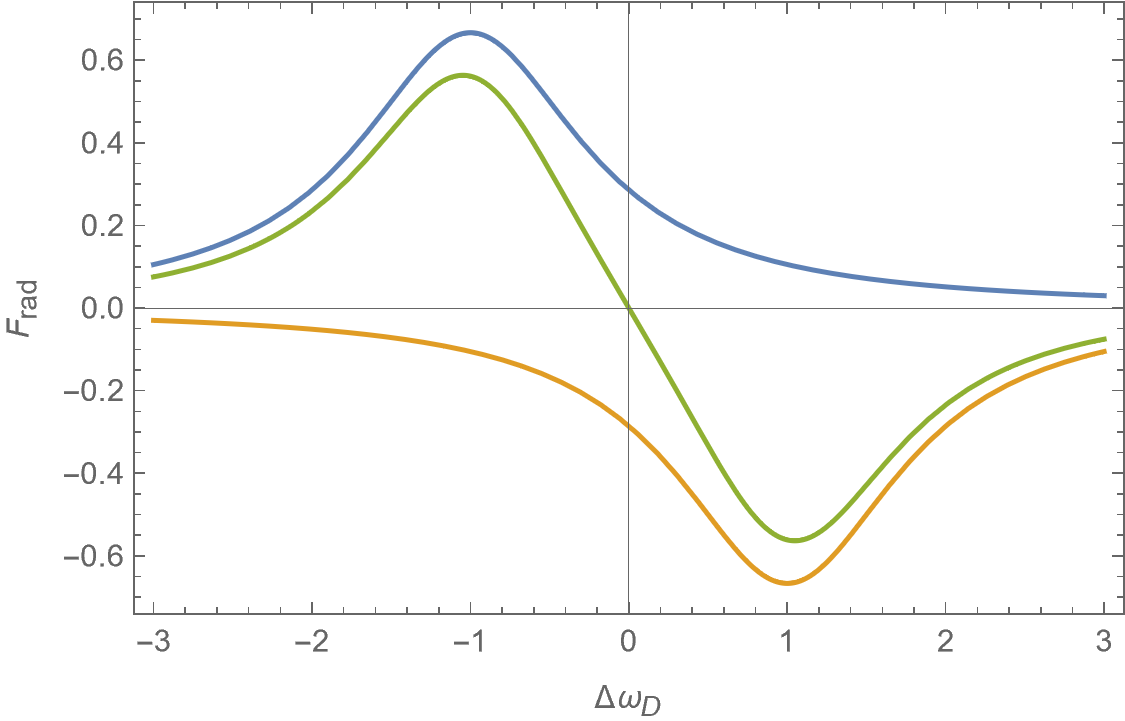
\includegraphics[width=0.45\textwidth]{Optical Molasses force1}
        \label{fig. Optical Molasses force1}}           
    \end{subfloat}
    \hfill
    \begin{subfloat}[]
        {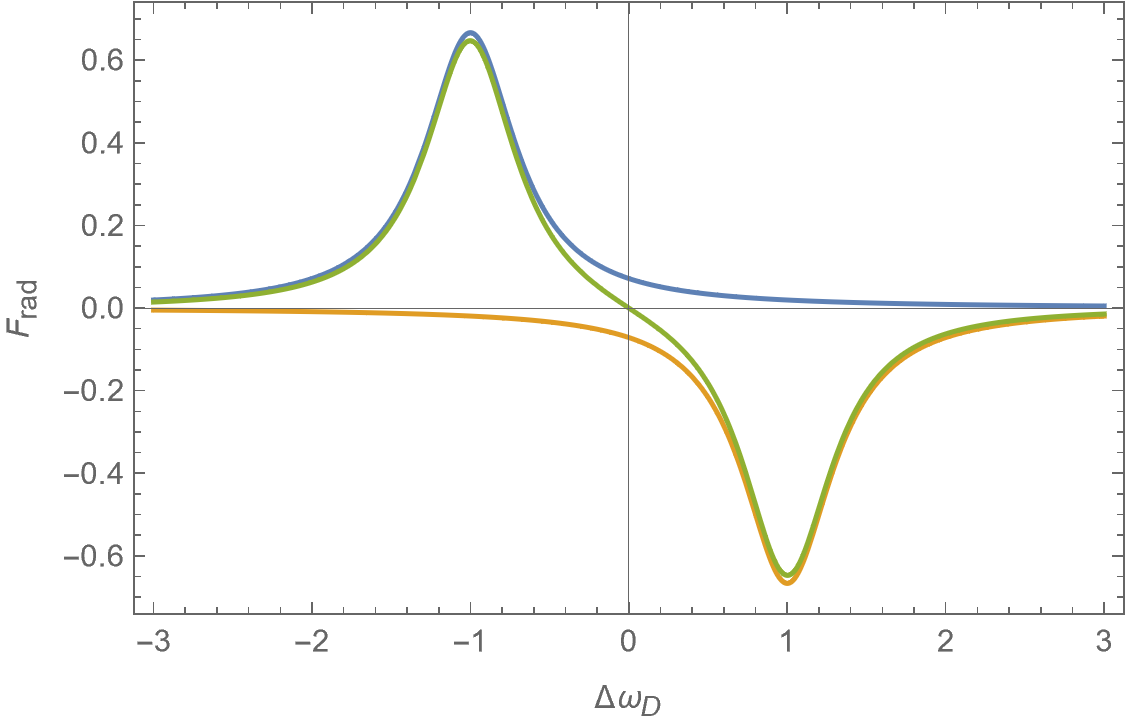
\includegraphics[width=0.45\textwidth]{Optical Molasses force2}
        \label{fig. Optical Molasses force2}}           
    \end{subfloat}
    \caption{The force from the two counter-propagating beams and their combined force on the atom for two different values of $\Gamma$. In each case $s_0=2$ and $\delta=-1$ and the prefactor $\hbar k\Gamma/2$ has been set equal to unity. In (a) $\Gamma$=1 while in (b) $\Gamma=0.4$. The linear regime near the center of (a) represents a viscous damping force since $\Delta\omega_D$ is directly proportional to the atom's velocity. In (b) the force it still a damping force but, not directly proportional to the velocity, so Eq.~\ref{eq. force from counter propagating beams} does not hold for (b) while it does for (a).}
    \label{fig. Optical Molasses forces}
\end{figure}


\newpage
In Strontium, two transitions are used to cool atoms, the strong 461 nm line coupling the $^1S_0-^1P_1$ states, and the much weaker 689 nm line coupling the $^1S_0-^3P_1$ states. 

\begin{figure}[H]
    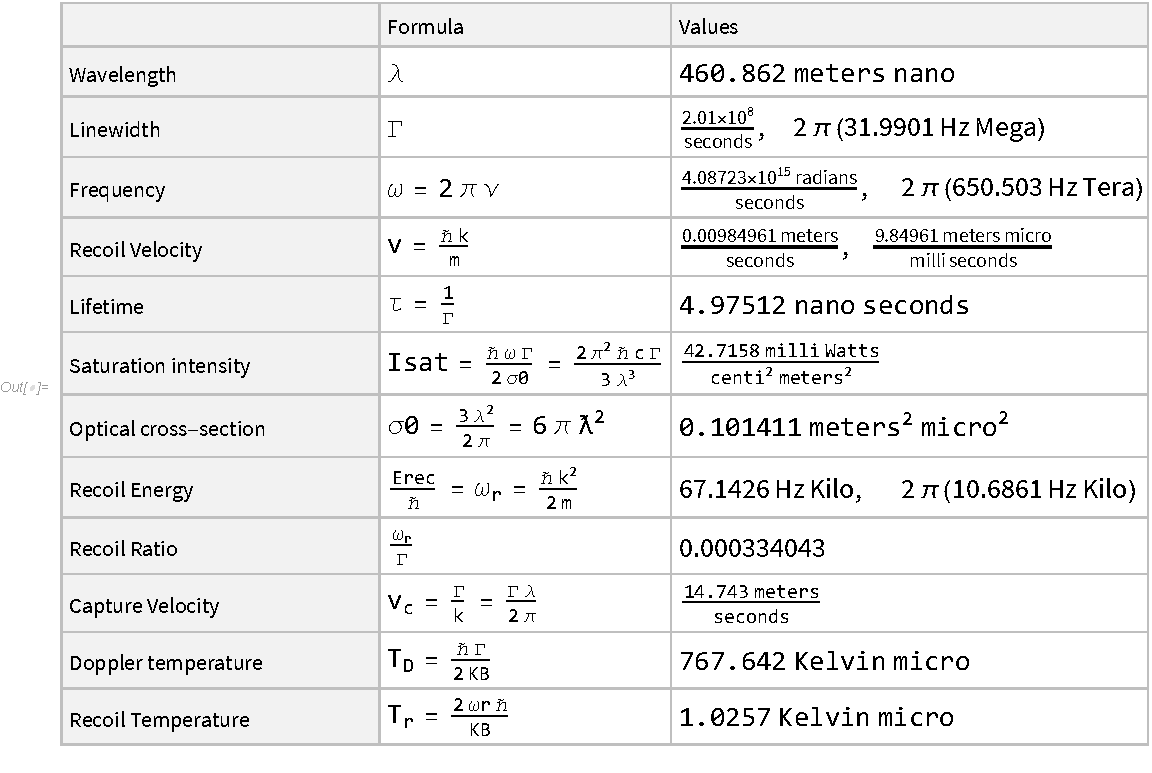
\includegraphics[width=\linewidth]{461table2}
    \caption{Table of values for the 461 nm transition}
\end{figure}
\begin{figure}[H]
    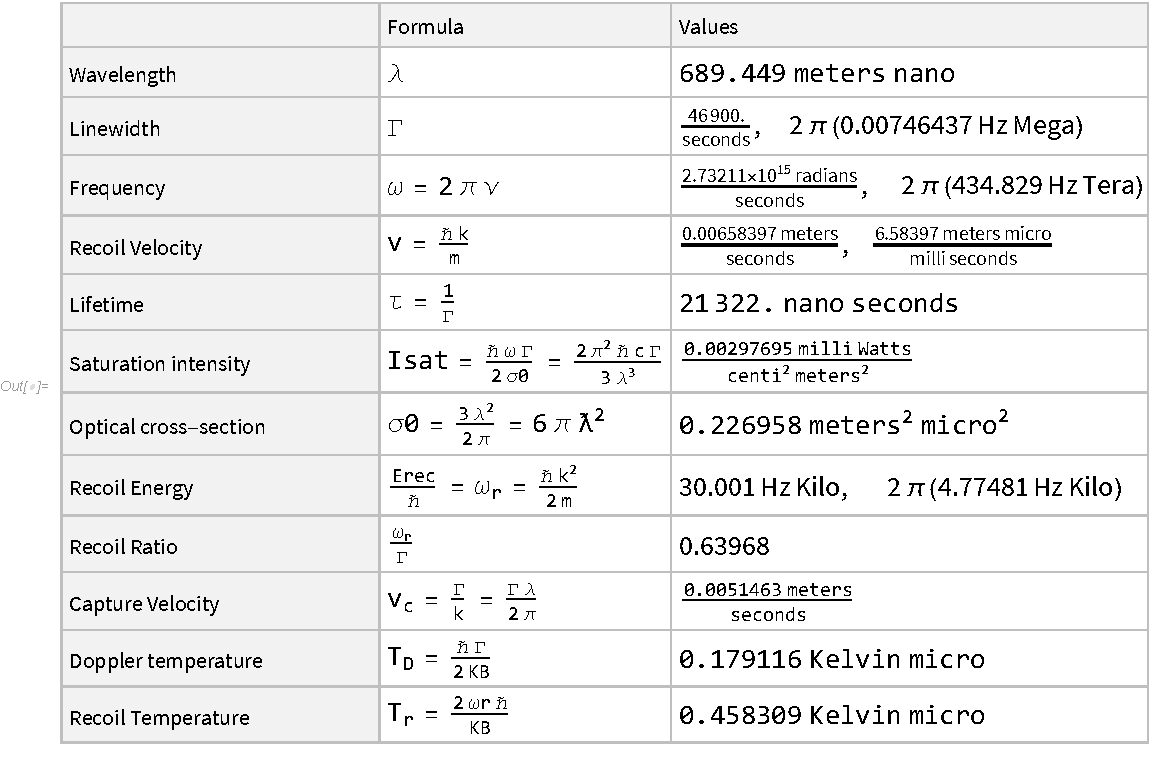
\includegraphics[width=\linewidth]{689table2}
    \caption{Table of values for the 698 nm transition}
\end{figure}


\end{document}